\documentclass{beamer}
\usetheme[everytitleformat=regular]{m}

\usepackage{graphicx}



\title{Modelling Weekly Sales Patterns}
\date{18th August 2015}
\author{Pete Bunch}
\institute{}



\begin{document}

\maketitle

\section{Me}

\begin{frame}{A bit about me}
 \begin{itemize}
  \item Recently moved to Austin from Cambridge, UK
  \item PhD in Statistical Signal Processing from University of Cambridge
 \end{itemize}
 \begin{center}
 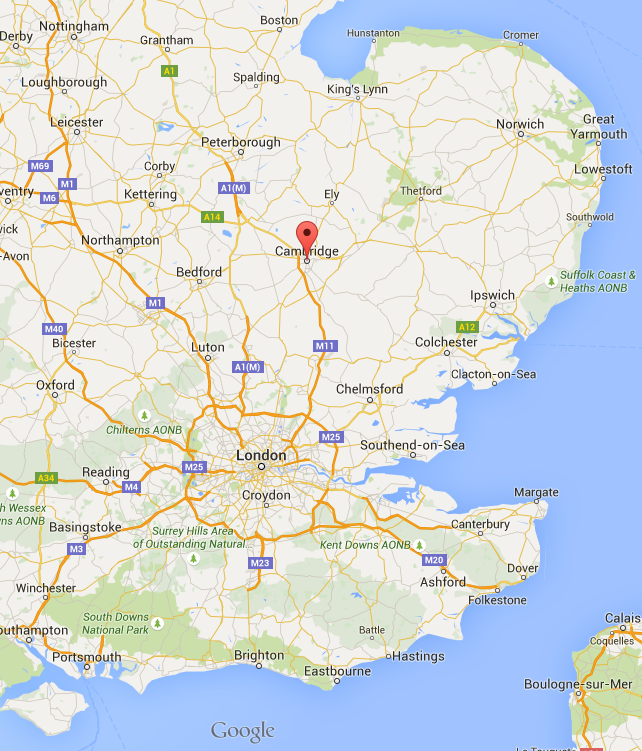
\includegraphics[width=0.3\columnwidth]{map.png} \qquad
 
\includegraphics[width=0.3\columnwidth]{cambridge.jpg} 
 \end{center}
\end{frame}

\begin{frame}{A bit about me}
 \begin{itemize}
  \item Far too much time in boats
 \end{itemize}
  \begin{center}
 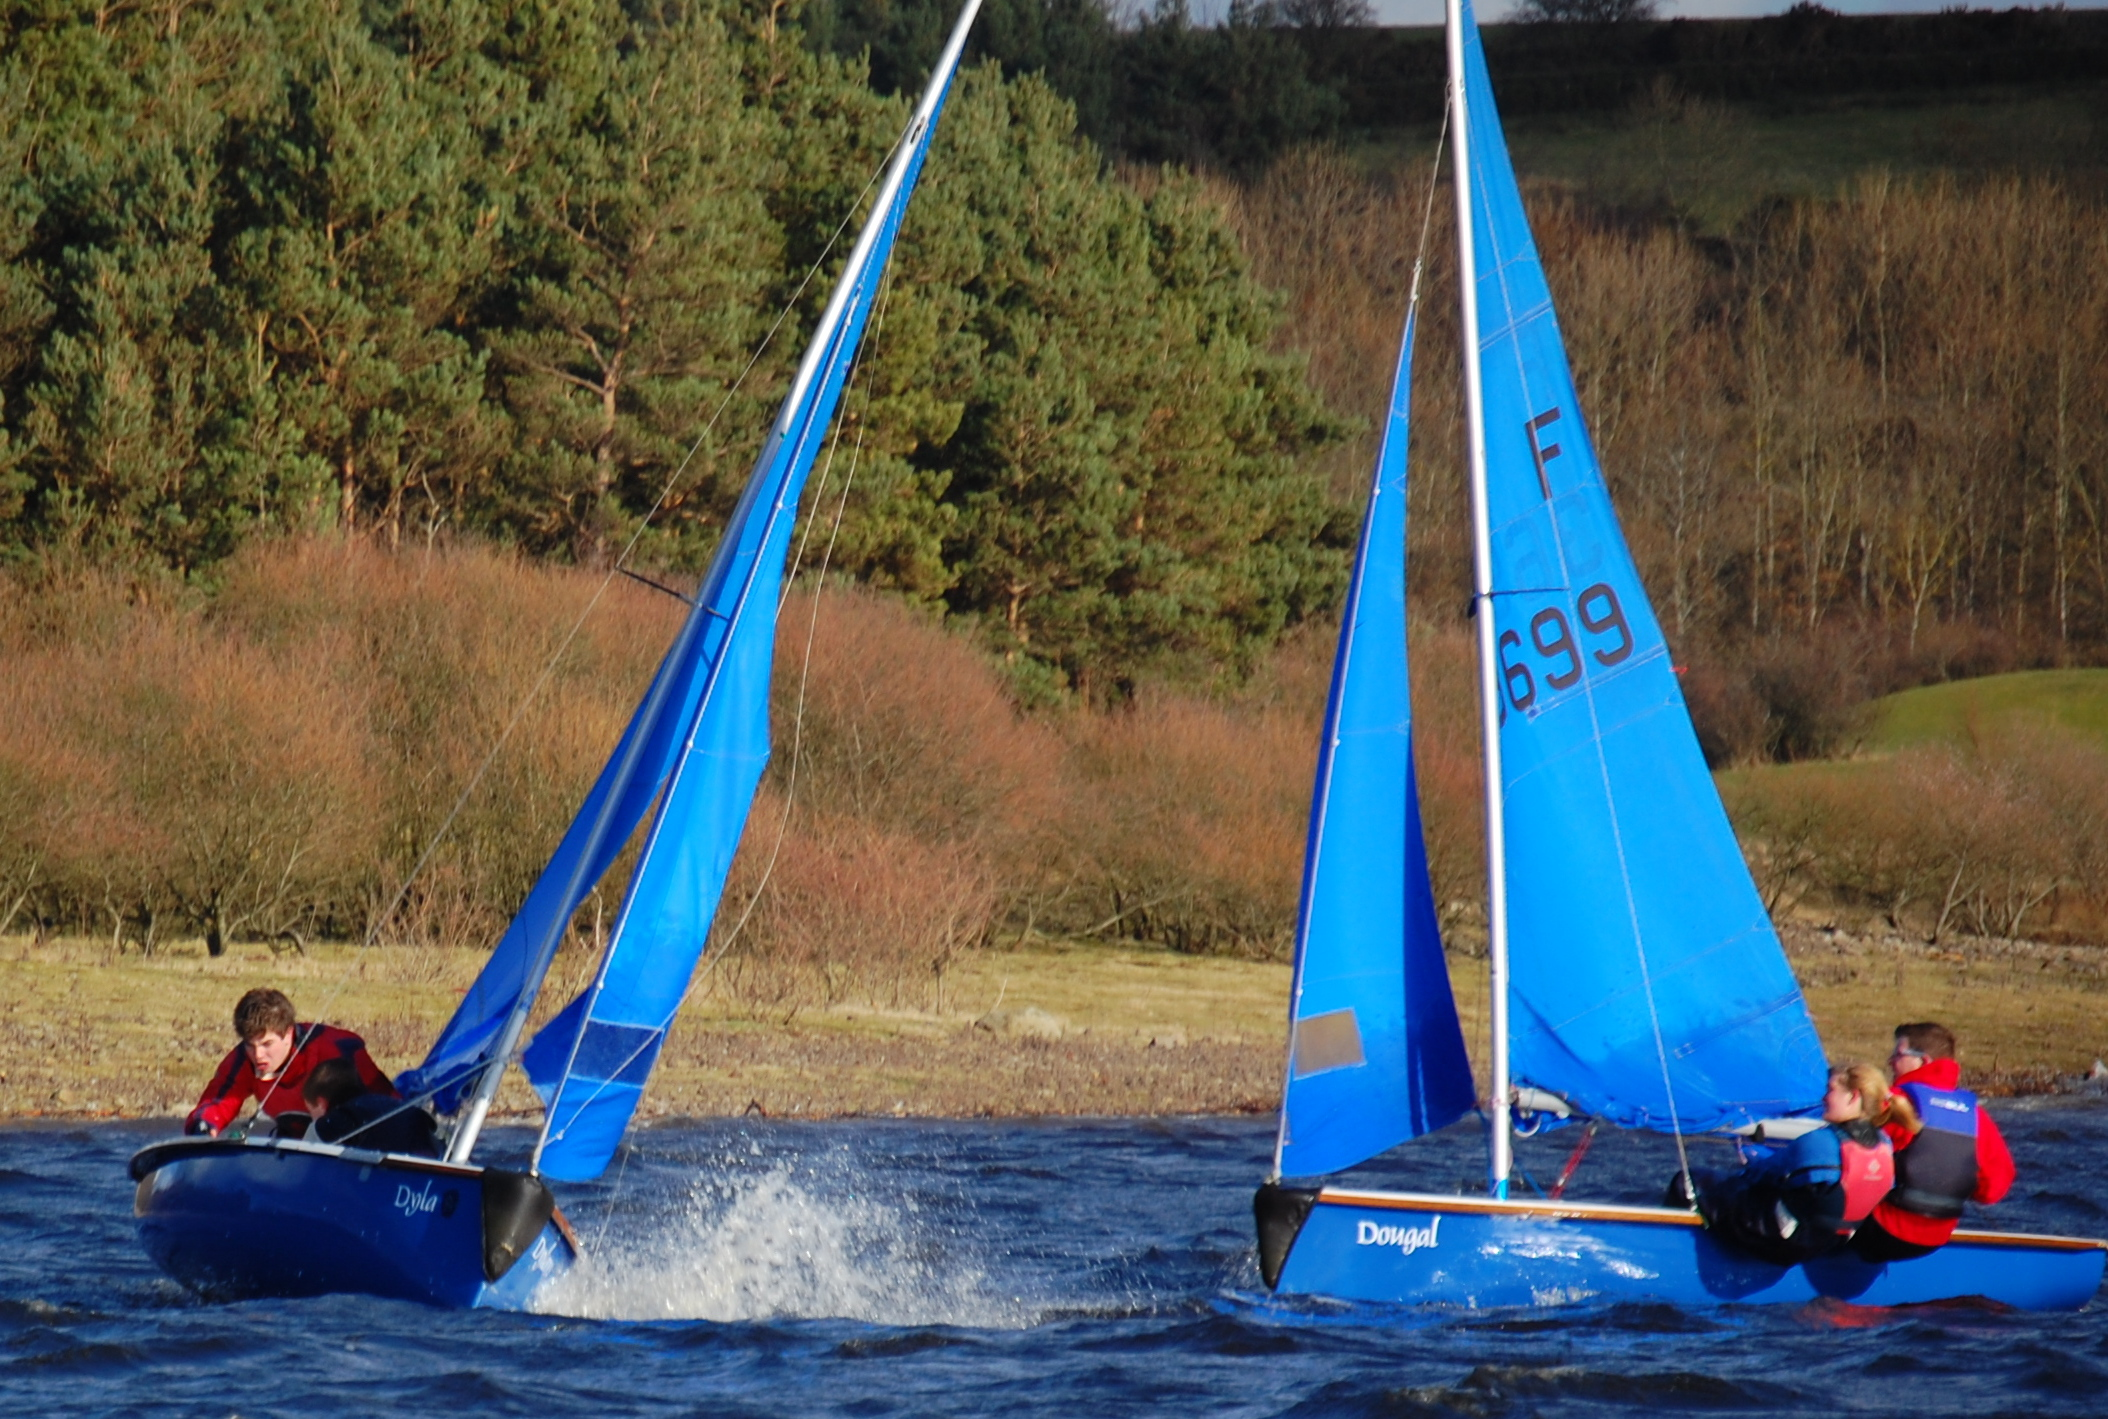
\includegraphics[height=0.3\columnwidth]{sailing.jpg} \qquad
 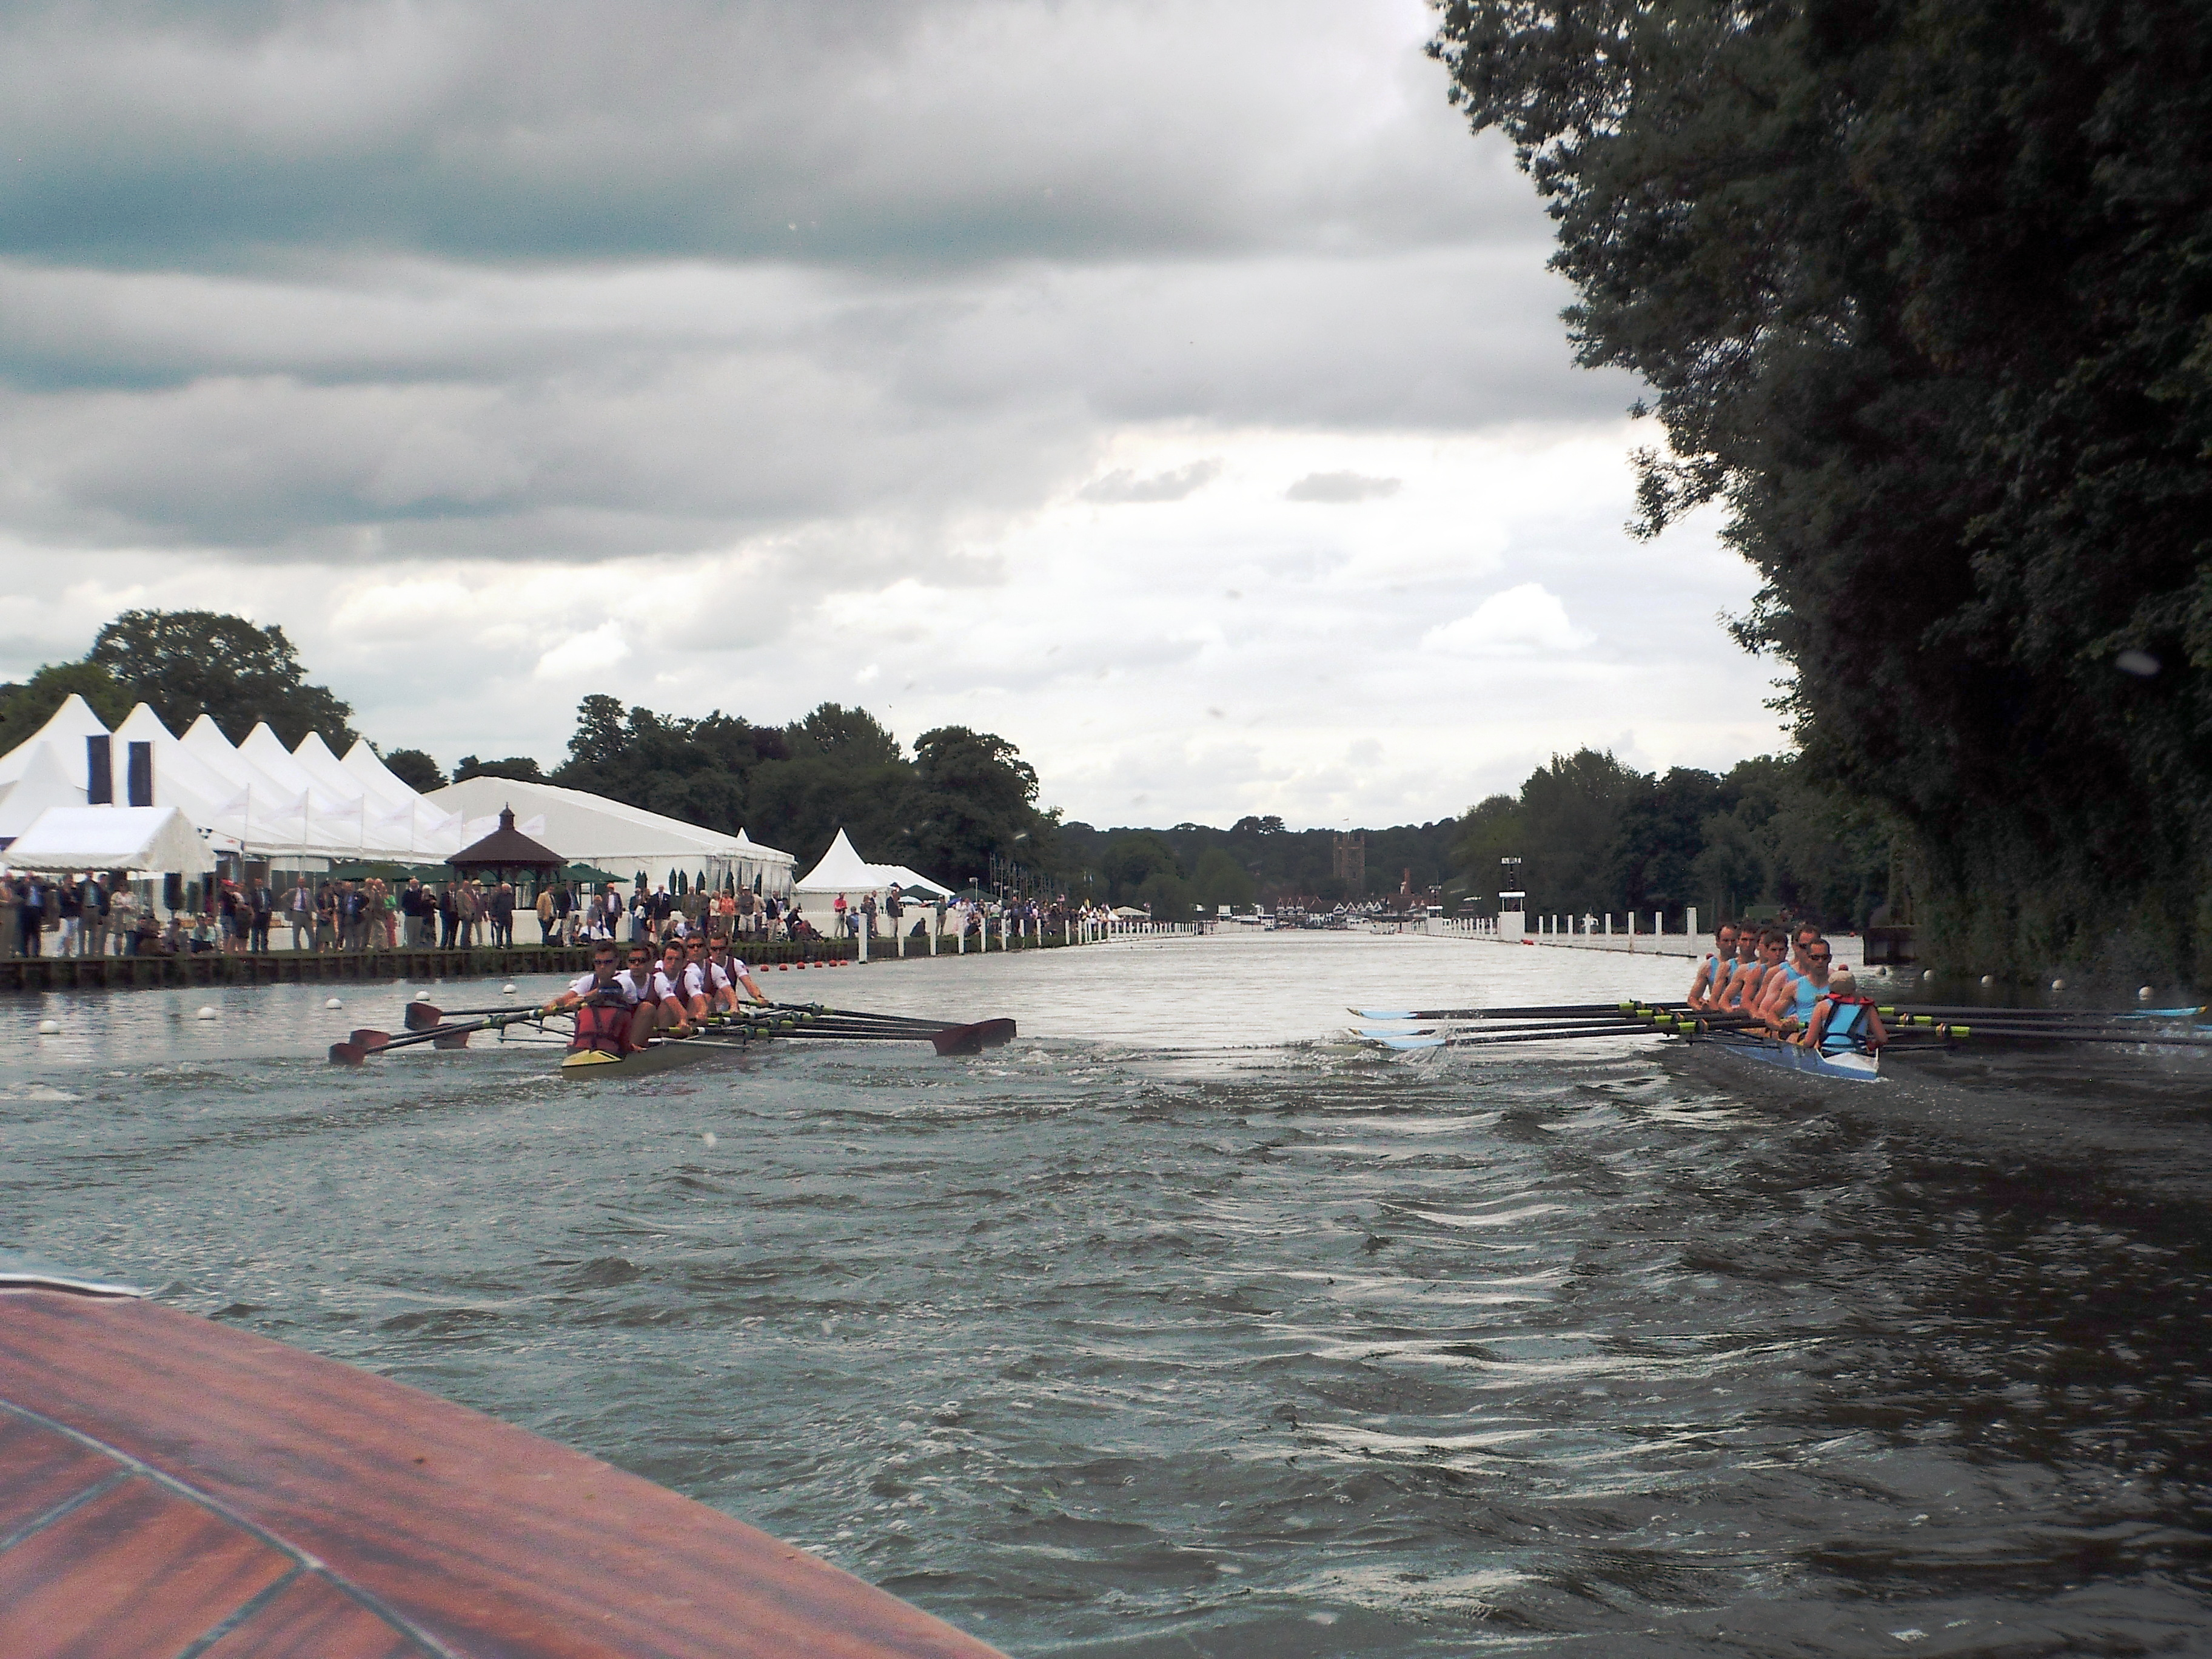
\includegraphics[height=0.3\columnwidth]{rowing.jpg} 
 \end{center}
\end{frame}

\begin{frame}{A bit about me}
  \begin{itemize}
  \item Pointless pet projects
 \end{itemize}
  \begin{center}
 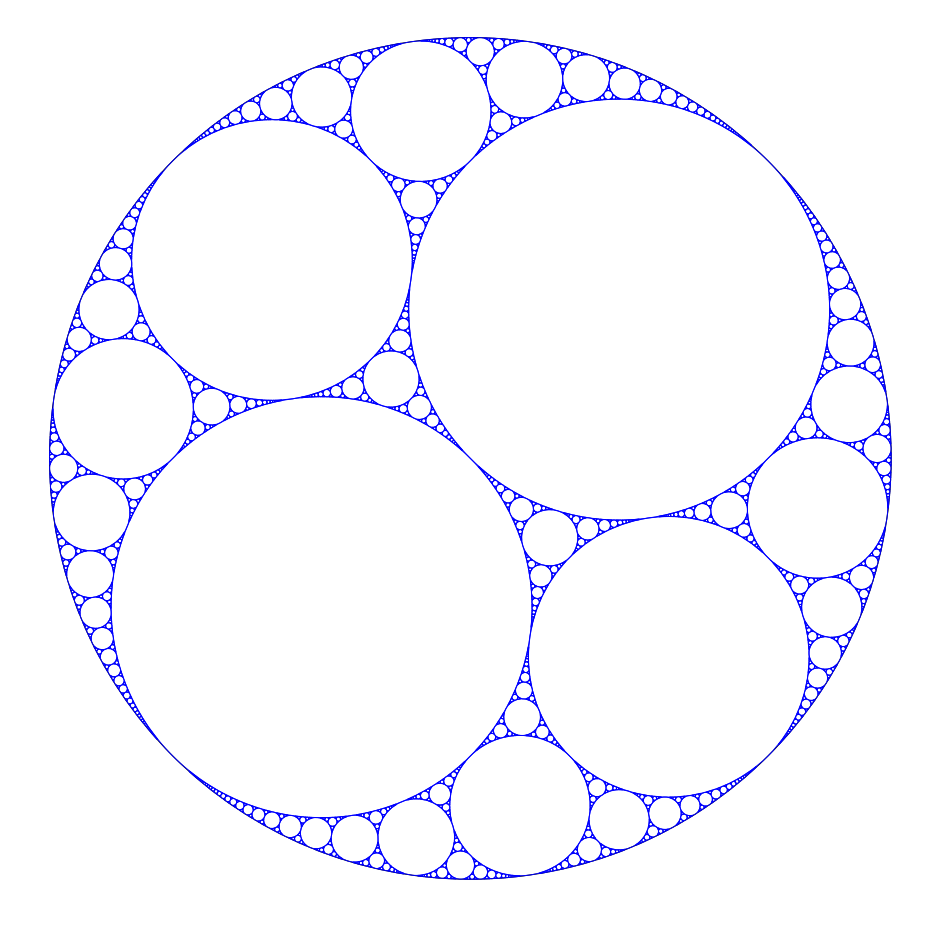
\includegraphics[height=0.3\columnwidth]{fractal.png} \qquad
 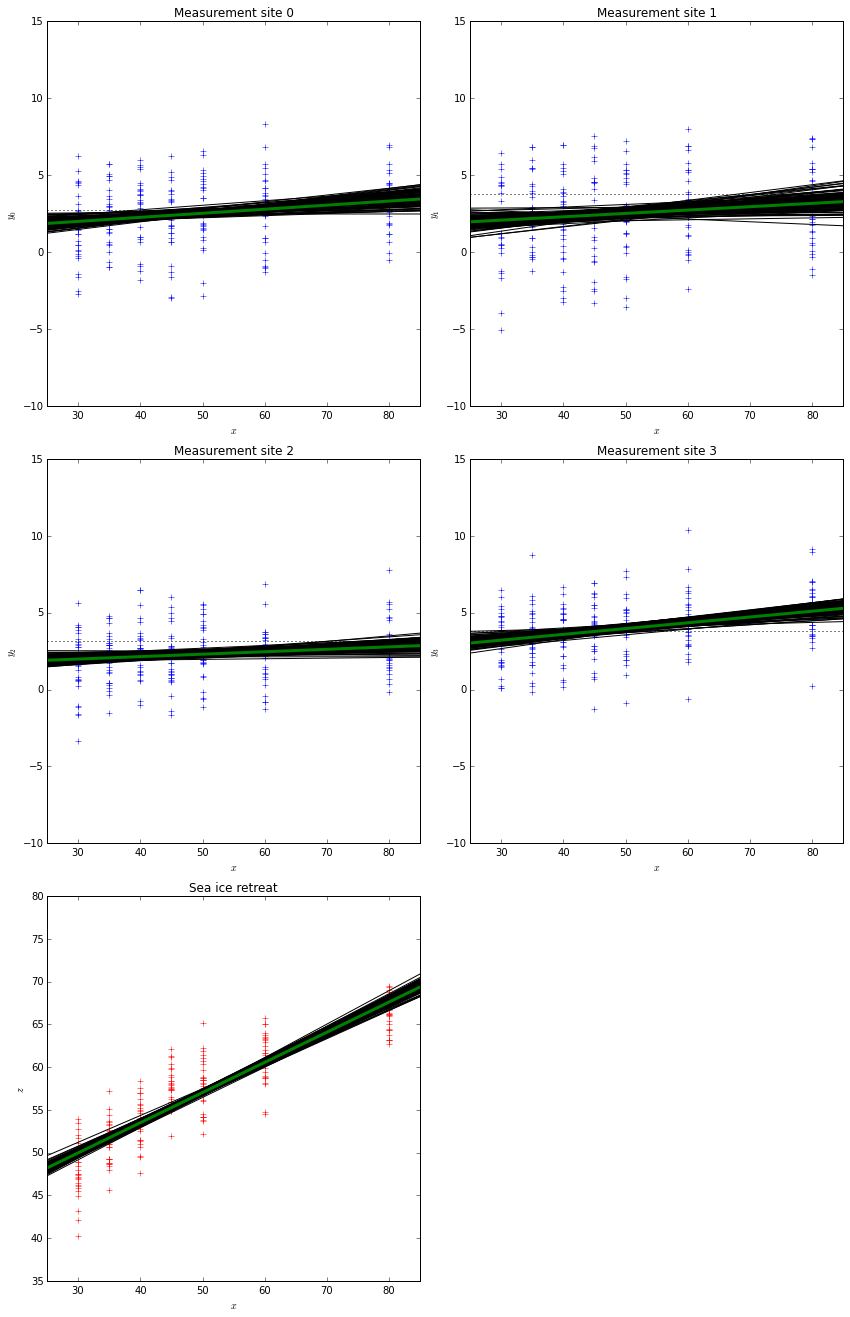
\includegraphics[height=0.3\columnwidth]{icecores.png} \\
 
\includegraphics[width=0.8\columnwidth]{blacklocus.png}
 \end{center}
\end{frame}


\section{Tesco Sales Modelling}

\begin{frame}{Tesco}
 \begin{itemize}
  \item Largest supermarket chain in the UK (28\% market share)
  \item Over 3,000 stores, operating in all regions
  \item Average of 10,000 products in each store
  \item Prediction for each product in each store, out to three weeks in advance
  \item Weather, promotions, events, reductions, seasonal patterns
  \item My focus: weekly patterns
 \end{itemize}
\end{frame}

\begin{frame}{Why does it matter?}
 \begin{itemize}
  \item Waste
  \item Stockholding
  \item Supplier interactions
 \end{itemize}
\end{frame}

\begin{frame}{Sales data: a ``fast'' seller}
 \begin{center}
  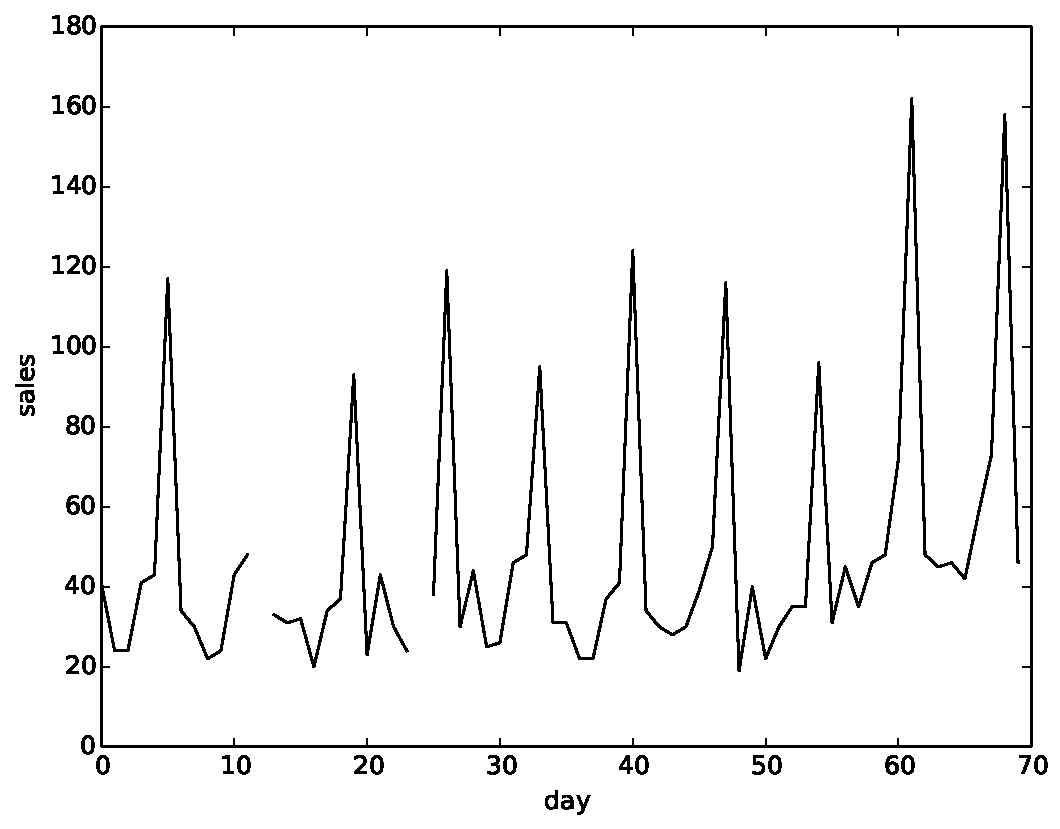
\includegraphics[width=0.8\columnwidth]{fast_seller.pdf}
 \end{center}
\end{frame}

\begin{frame}{Sales data: a ``medium'' seller}
 \begin{center}
  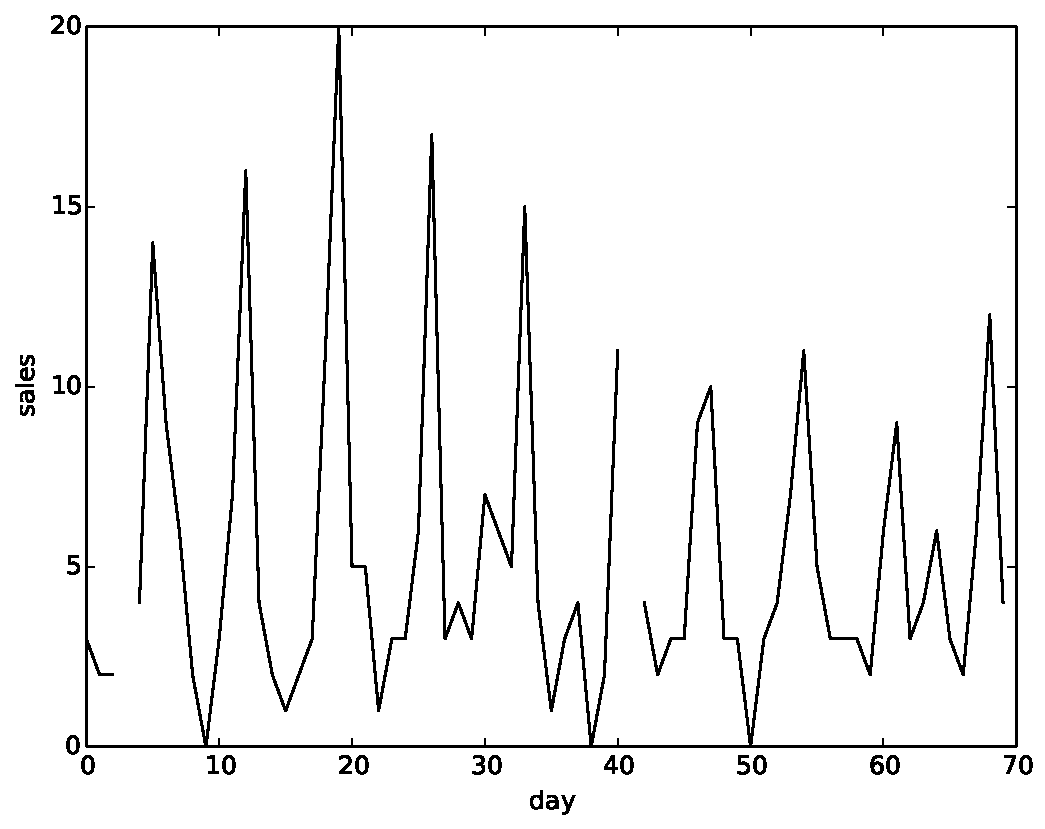
\includegraphics[width=0.8\columnwidth]{medium_seller.pdf}
 \end{center}
\end{frame}

\begin{frame}{Sales data: a ``slow'' seller}
  \begin{center}
  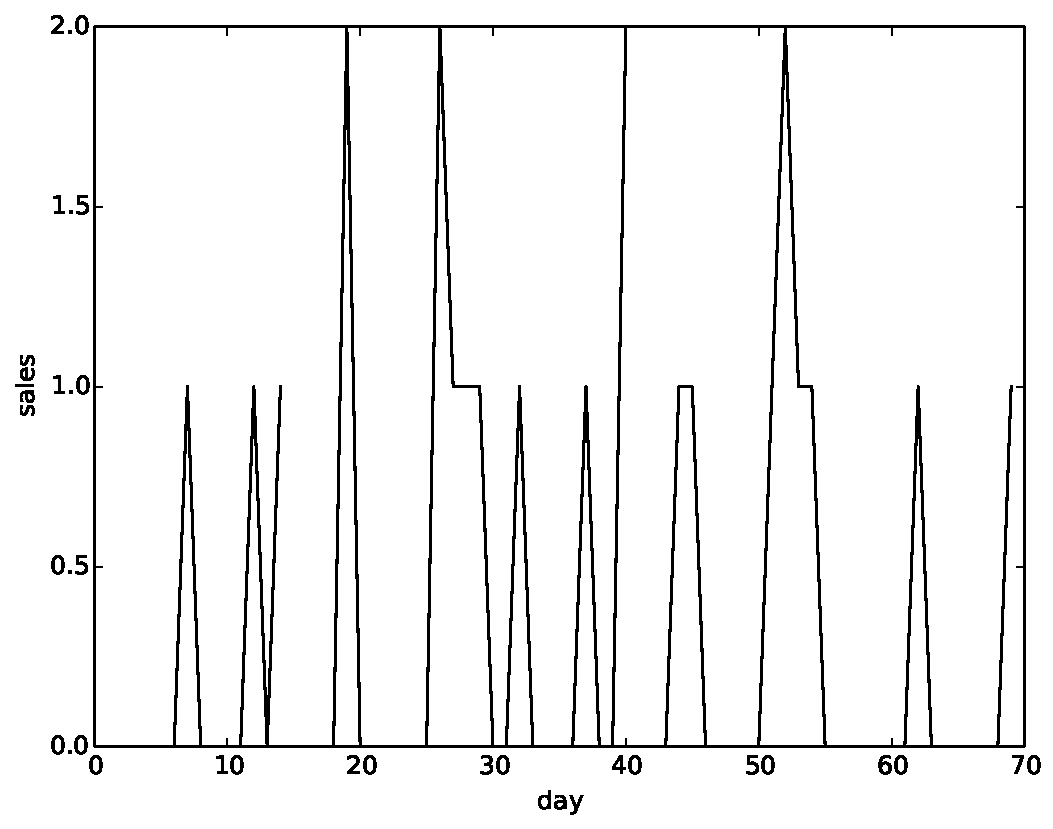
\includegraphics[width=0.8\columnwidth]{slow_seller.pdf}
 \end{center}
\end{frame}

\begin{frame}{Sales model: single-product, single-store}
 \begin{equation}
  x_{ij} \underset{\text{\tiny i.i.d.}}{\sim} \mathcal{P}(u_i \cdot v_j)
 \end{equation}
 \begin{tabular}{ll}
  $x_{ij}$ & sales on day $i$ of week $j$ \\
  $v_j$    & expected sales in week $j$ \\
  $u_i$    & proportion of sales on day $i$
 \end{tabular}
 \begin{equation}
  \begin{bmatrix} \; & & \; \\ & X & \\ & & \end{bmatrix} \sim \begin{bmatrix} \vdots \\ U \\ \vdots \end{bmatrix} \times \begin{bmatrix} \cdots & V & \cdots \end{bmatrix}
 \end{equation}
 \begin{equation}
  \sum_i u_i = 1
 \end{equation}
\end{frame}

\begin{frame}{Sales model: single-product, single-store}
 \begin{center}
  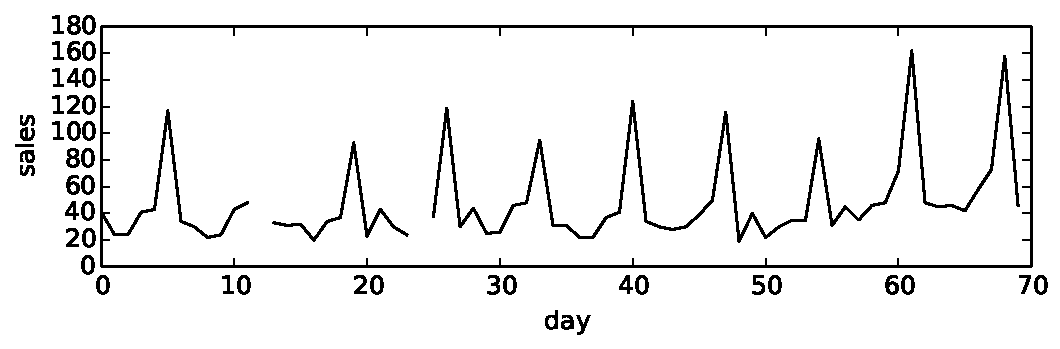
\includegraphics[width=0.8\columnwidth]{fast_seller_small.pdf} \\
  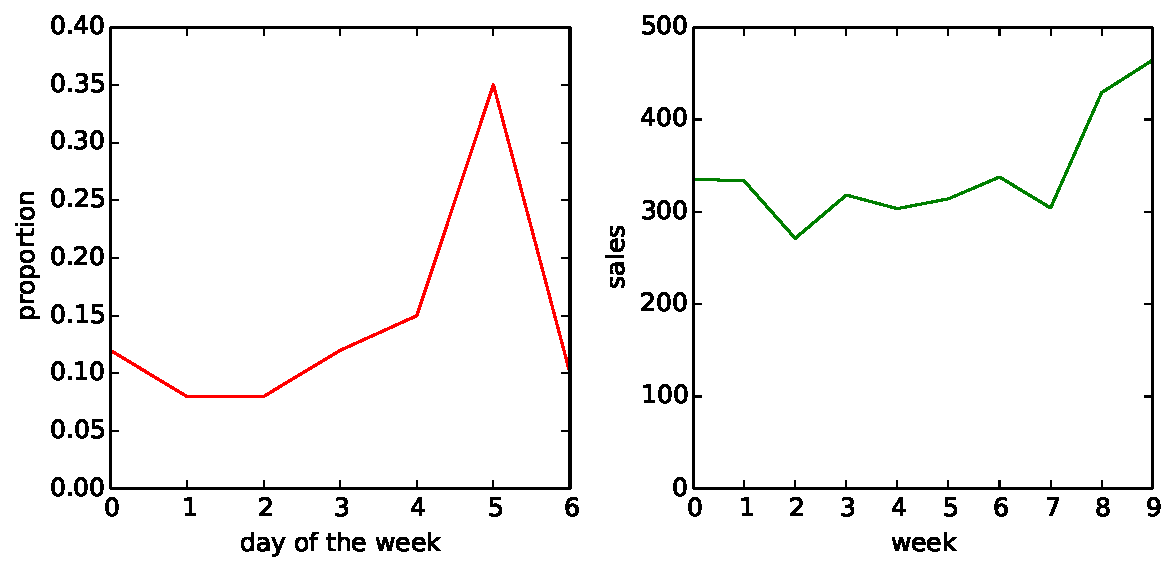
\includegraphics[width=0.8\columnwidth]{fast_factorisation.pdf}
 \end{center}
\end{frame}

\begin{frame}{Fitting: maximum likelihood}
 Mask variables: $m_{ij} \in \{0,1\}$
 \vspace{0.5cm}
 
 Log-likelihood:
 \begin{align}
  %p(X|U,V) &= \prod_{i,j} \left[\frac{ \exp(-u_i v_j) (u_i v_j)^{x_{ij}} }{ x_{ij}! }\right]^{m_{ij}} \\
  \mathcal{L}(U,V) &= \sum_{i,j} m_{ij} \left[ -u_i v_j + x_{ij}\log(u_i v_j) - \log(x_{ij}!) \right]
 \end{align}
 
 Maximize iteratively:
 \begin{align}
  u_i &\leftarrow \frac{\sum_j x_{ij} m_{ij}}{\sum_j v_{j} m_{ij}} & \qquad v_j &\leftarrow \frac{\sum_i x_{ij} m_{ij}}{\sum_j u_{i} m_{ij}}
 \end{align}
\end{frame}

\begin{frame}{Fast seller training}
  \begin{center}
  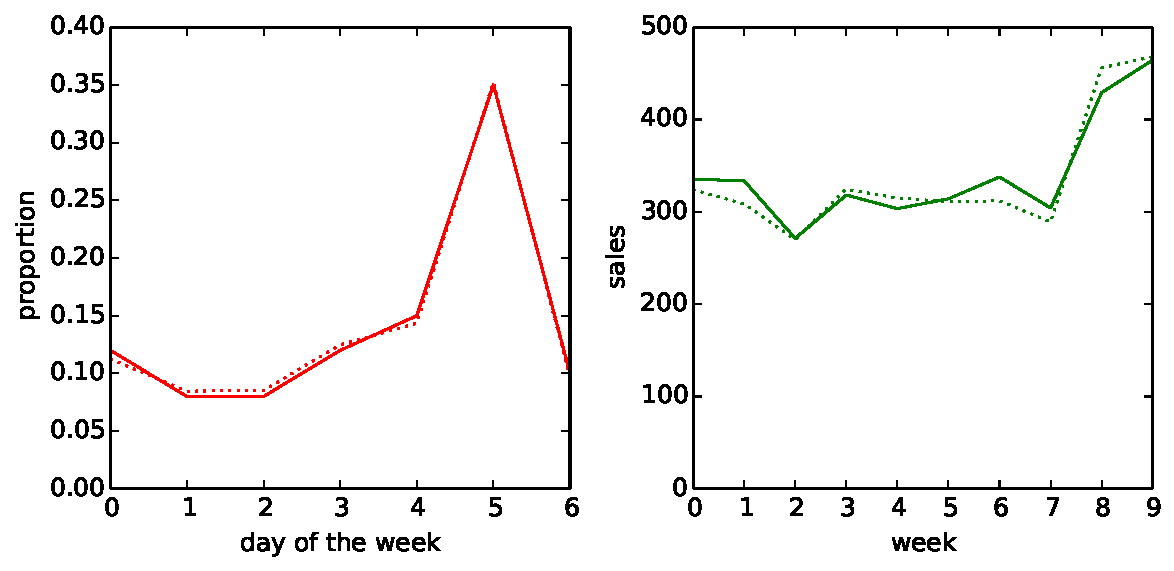
\includegraphics[width=0.8\columnwidth]{fast_learning.pdf}
 \end{center}
\end{frame}

\begin{frame}{Medium seller training}
  \begin{center}
  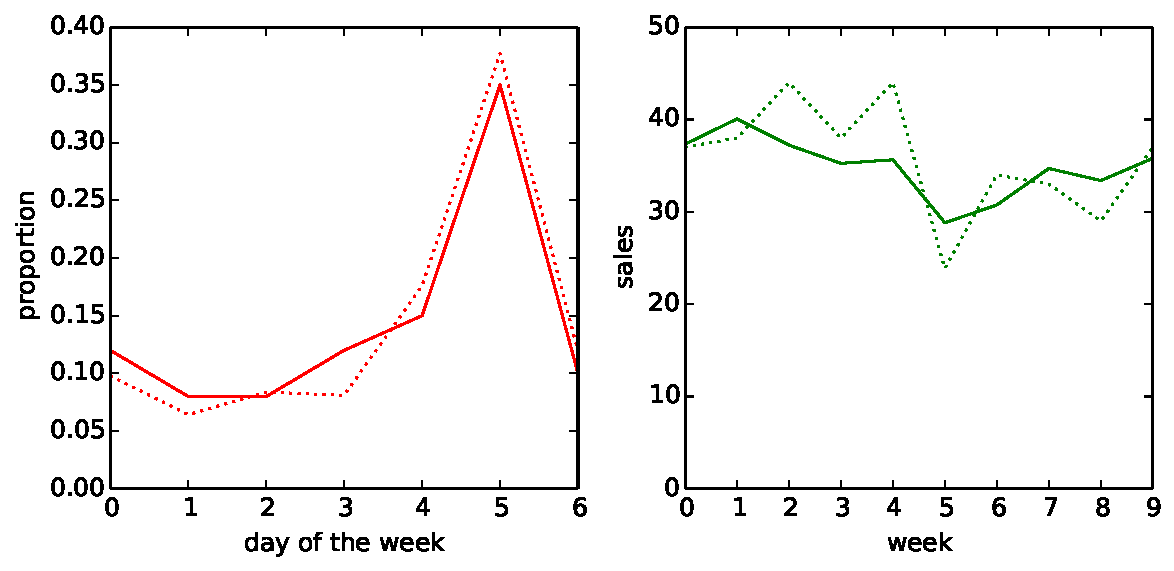
\includegraphics[width=0.8\columnwidth]{medium_learning.pdf}
 \end{center}
\end{frame}

\begin{frame}{Slow seller training}
  \begin{center}
  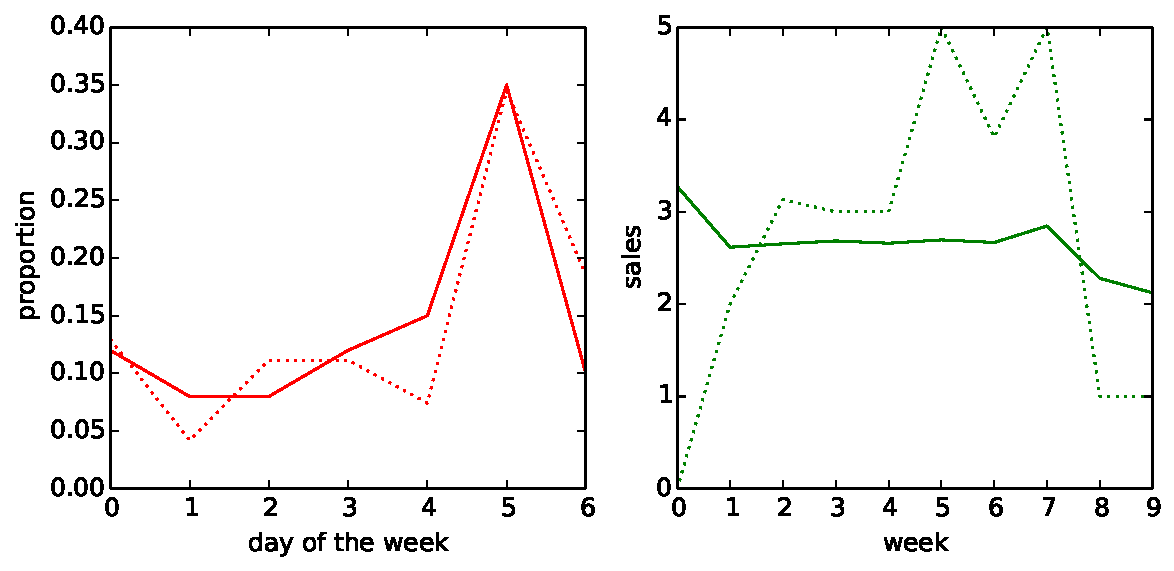
\includegraphics[width=0.8\columnwidth]{slow_learning.pdf}
 \end{center}
\end{frame}

\begin{frame}{Sales model: single-store, multiple products}
 \begin{equation}
  x_{ij}^{(n)} \underset{\text{\tiny i.i.d.}}{\sim} \mathcal{P}\left(u_i^{(z_n)} \cdot v_j^{(n,z_n)}\right)
 \end{equation}
 \begin{tabular}{ll}
  $x_{ij}^{(n)}$ & sales of product $n$ on day $i$ of week $j$ \\
  $u_i^{(k)}$    & proportion of sales on day $i$ for products in cluster $k$ \\
  $v_j^{(n,k)}$  & expected sales of product $n$ in week $j$, \\
                 & \qquad estimated as if it were in cluster $k$ \\
  $z_n$          & cluster indicator for product $n$
 \end{tabular}
\end{frame}

\begin{frame}{Fitting: maximum likelihood}
 Log-likelihood:
 \begin{align}
  \mathcal{L}(U,V,Z) &= \sum_{i,j,n} m_{i,j}^{(n)} \bigg[ -u_i^{(z_n)} v_j^{(n,z_n)} + x_{ij}^{(n)}\log(u_i^{(z_n)} v_j^{(n,z_n)}) \nonumber \\
  &\qquad\qquad\qquad\qquad\qquad\qquad -\: \log(x_{ij}^{(n)}!) \bigg]
 \end{align}
 
 \begin{itemize}
  \item $V$ update unchanged
  \item $U$ update uses all products in the cluster
  \item $Z$ update by assigning each product to the cluster which maximises the likelihood
 \end{itemize}
 Tendency to get stuck in local maxima. Sensitive to starting conditions.
\end{frame}

\begin{frame}{Better fitting: expectation maximisation}
 Marginal log-likelihood:
 \begin{align}
  \mathcal{L}(U,V) &= \log\left(\sum_Z p(X|U,V,Z) p(Z)\right)
 \end{align}
 \begin{itemize}
  \item Lower bound the marginal log-likelihood
  \item Bound depends on $p(Z|X,U,V) = \prod_n p(z_n|X,U,V)$
  \item Soft clustering
 \end{itemize}
\end{frame}

\begin{frame}{Further details}
 \begin{itemize}
  \item Common clustering over multiple stores
  \item Probabilistic outlier detection
  \item Train on a rolling window every few weeks
  \item Implemented in SQL (with MATLAB)
  \item Sales are not Poisson distributed. Model over-dispersion.
 \end{itemize}
\end{frame}

\begin{frame}{Does it work?}
 \begin{itemize}
  \item Yes
  \item $1$--$2\%$ improvement in forecast accuracy metrics
  \item Estimated \pounds(some millions) in fresh food waste per year
 \end{itemize}
\end{frame}

\section{BlackLocus Sales Modelling Challege}

\begin{frame}{Forecast sales for 2015}
 \begin{center}
  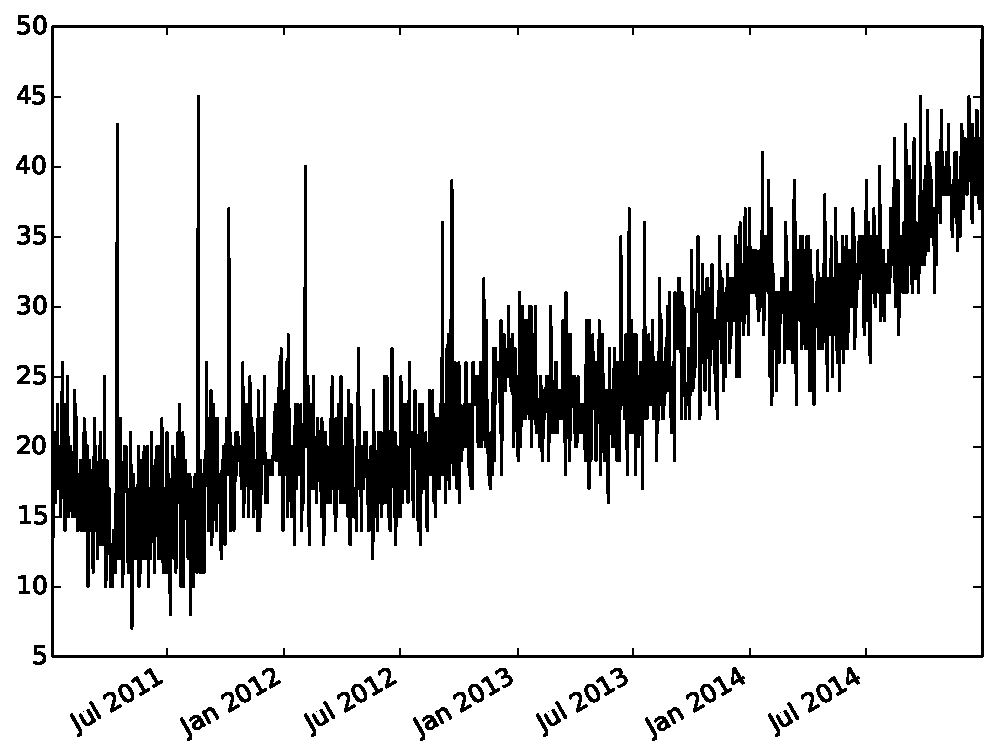
\includegraphics[width=0.8\columnwidth]{sales.pdf}
 \end{center}
\end{frame}

\begin{frame}{Another Poisson model}
 \begin{equation}
  x_{t} \underset{\text{\tiny i.i.d.}}{\sim} \mathcal{P}(f_t \cdot g_t)
 \end{equation}
 
 \begin{tabular}{ll}
  $f_t$ & Linear combination of polynomial basis functions \\
  $g_t$ & Linear combination of Fourier series basis functions (yearly period)
 \end{tabular}
 
 \begin{itemize}
  \item Maximise likelihood by gradient ascent (Newton's method)
  \item Choose model orders by cross-validation (train on 2011-2013, assess on 2014)
  \item Linear trend extrapolation
 \end{itemize}
\end{frame}

\begin{frame}{Forecast sales for 2015}
 \begin{center}
  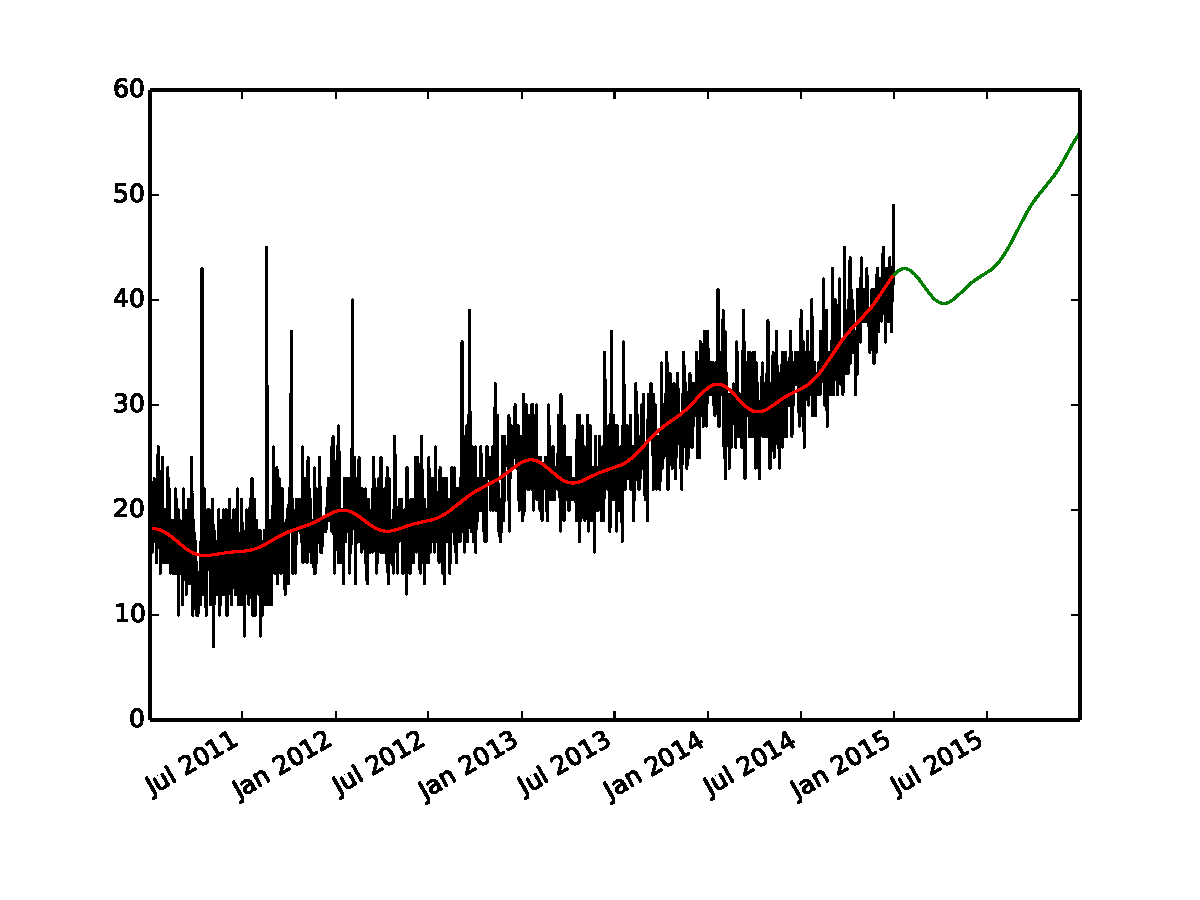
\includegraphics[width=0.8\columnwidth]{modelled.pdf}
 \end{center}
\end{frame}

\begin{frame}{If I had more time...}
 \begin{itemize}
  \item Learn distribution over parameters and marginalise (MCMC)
  \item Model and remove outliers
  \item Check Poisson assumption
 \end{itemize}
\end{frame}

\begin{frame}
\end{frame}



\end{document}


